In this section we report our numerical results. We start by showing how the baseline data benchmark presented in \cite{shenoy2026uncertainty} is affected by epistemic uncertainty, and how our proposed approach can mitigate its impact. Furthermore, we propose a more nuanced version of their benchmark, where the detection task at end is more challenging, further highlighting the validity of our mitigation approach in less ad-hoc settings. Finally, we present a real-world case study of a medical device, introducing a benchmark easily downloadable through Proto-OKN, demonstrating the practical applicability and benefits of our proposed method in a high-stakes setting.

\subsection{Synthetic Benchmark}
\label{subsec:synthetic-benchmark}
\begin{enumerate}
    \item \marco{Description of the data, in particular the fact the original synthetic data had very simple feature to separate the classes, and why we propose a more challegning benchmark.}
    \item \raham{Added pseudocode for dataset generation below - awaiting approval}
    \item \raham{We need a pseudocode of the benchmark generation, and a description of the parameters that can be tuned to make the benchmark more or less challenging. This will go in the appendix, but it will be referenced here.}
    \item \raham{Description of the model used for the experiments, and the training procedure.}
    \item \raham{Risk plots should be averaged over multiple runs, and the number of runs should be reported.}
\end{enumerate}

% \begin{figure*}
%     \centering
%     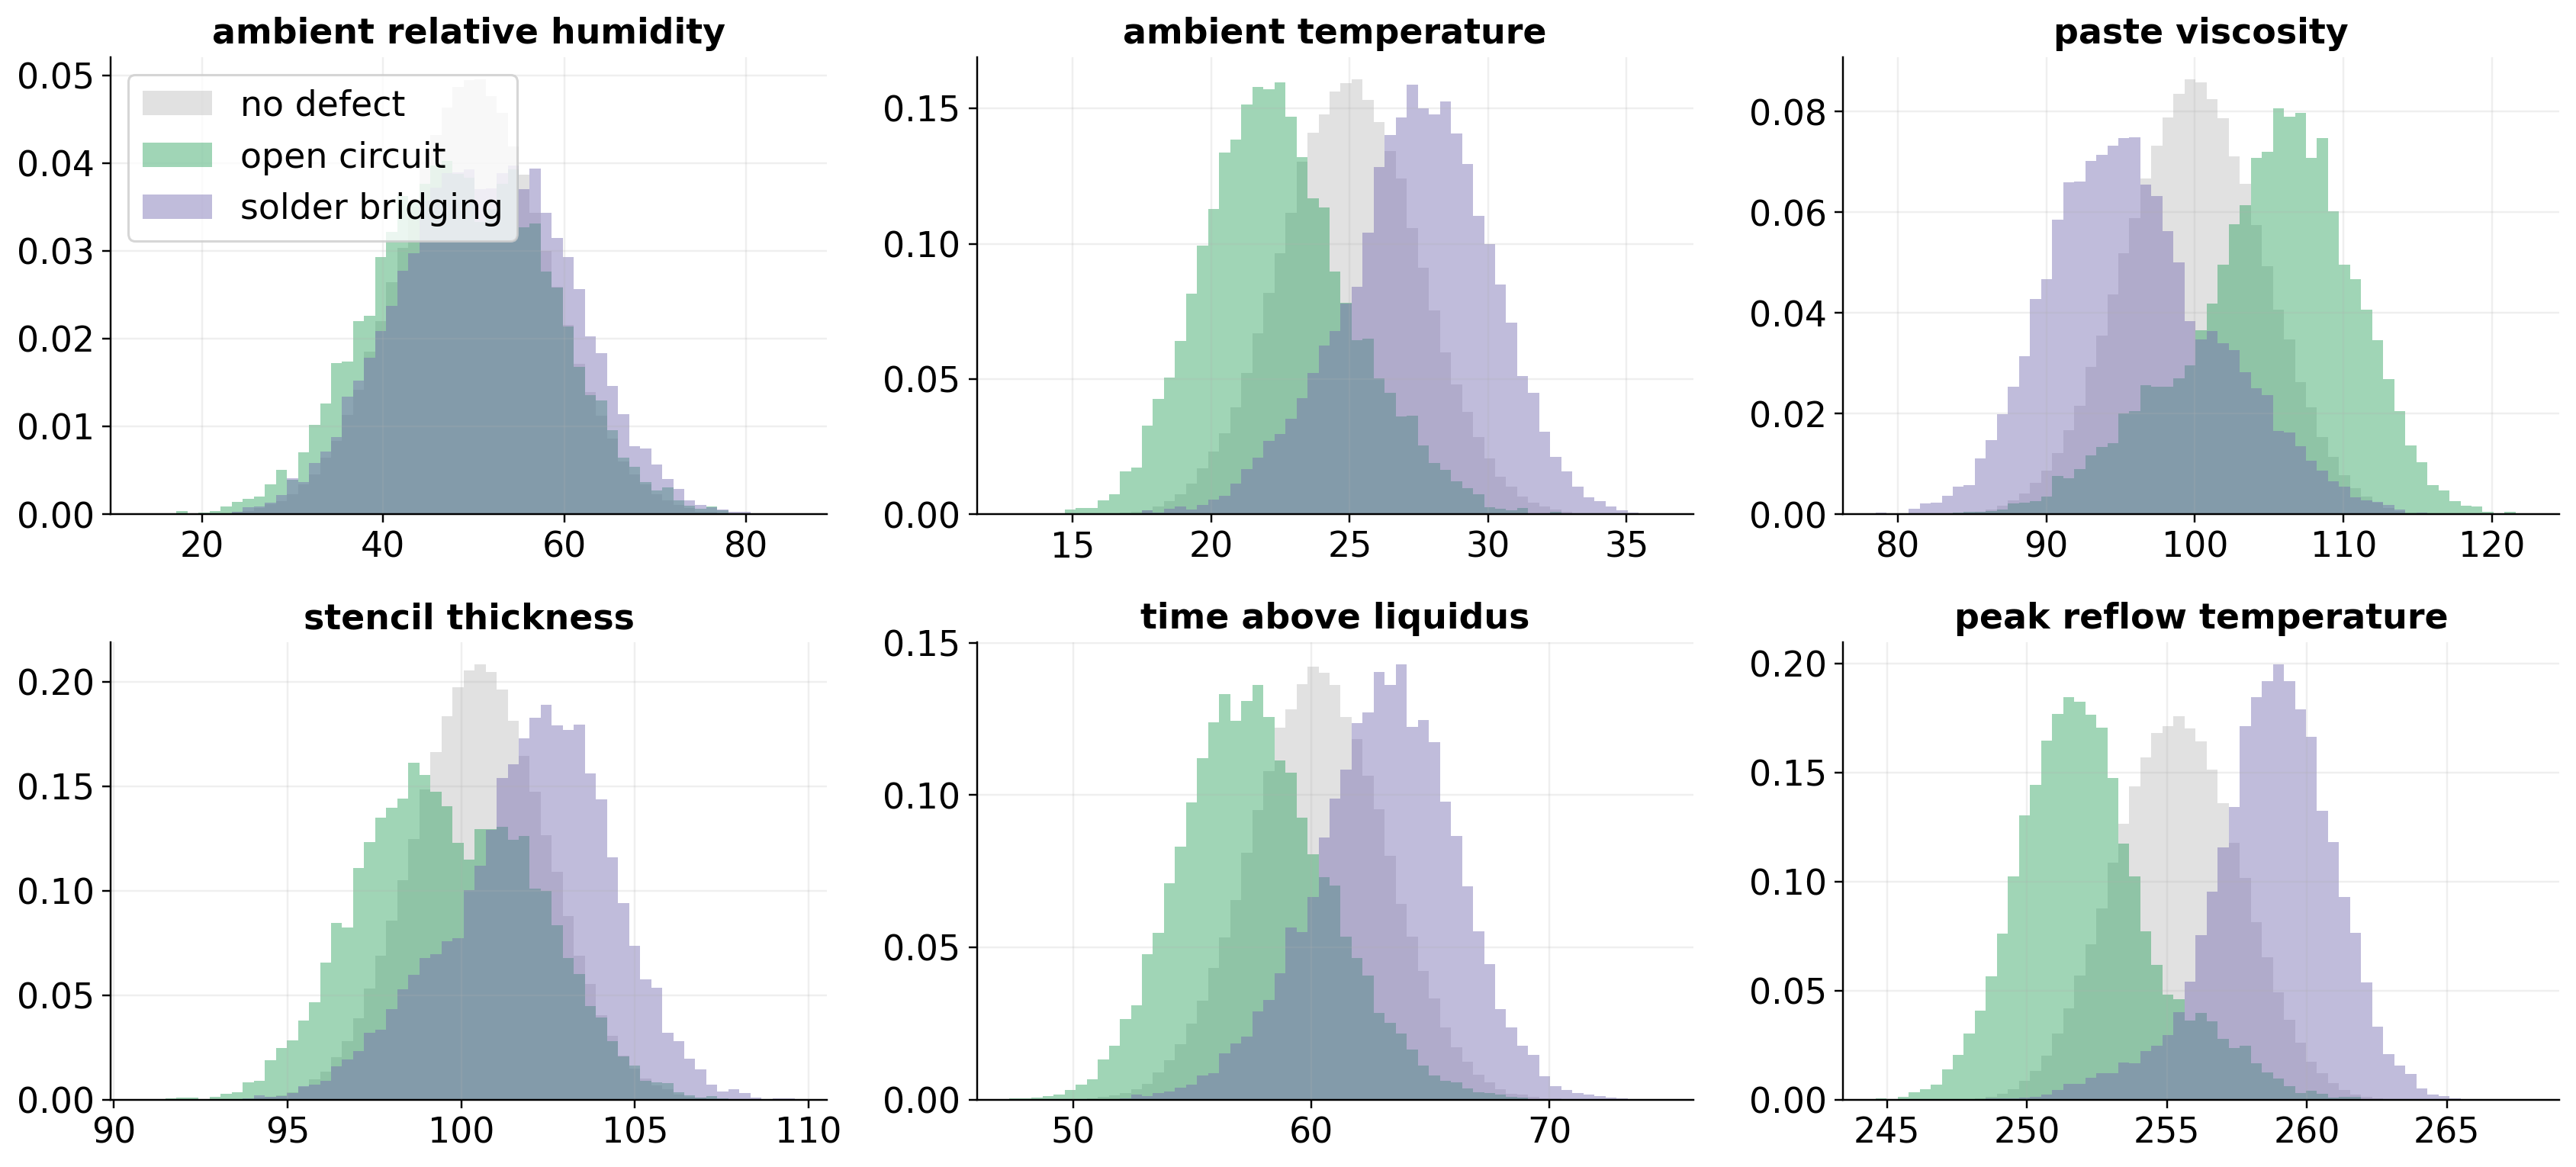
\includegraphics[scale=0.4]{../tex/img/fig_feature_separability_baseline.png}
% \end{figure*}

\begin{algorithm}[t]
\caption{Synthetic benchmark generation}
\label{alg:generator}
\DontPrintSemicolon
\SetKwInOut{Input}{Input}\SetKwInOut{Output}{Output}
\SetKwFunction{Cat}{Categorical}\SetKwFunction{Softmax}{softmax}
\Input{process spec (parameter targets, spreads, correlations, drift); a causal map of which parameters cause which defects; the class proportions; a target Bayes error $\varepsilon^\star$; a random seed}
\Output{labeled boards (each with its defect, mechanism, and per-parameter risk) split into train / validation / test}
\BlankLine
sample correlated process parameters for every board, adding slow tool wear and a daily cycle\;
measure how far each parameter drifts from its specification limits\;
score each defect $d$ from the parameters that cause it, giving $s_d(\x)$\;
form the class posterior, with the gain $\gamma$ tuned so the Bayes error equals $\varepsilon^\star$:
\[ \PYX(d\mid\x)=\Softmax\!\big(\gamma\,s_d(\x)+\beta_d\big) \]
draw each board's label $y \sim \Cat\big(\PYX(\cdot\mid\x)\big)$\tcp*{sampled, not thresholded}
tag the responsible mechanism and assign a graded risk to each parameter\;
split whole batches into train / validation / test and attach provenance\;
\Return the labeled, split dataset\;
\end{algorithm}

\begin{figure*}[t]
    \centering

    \begin{subfigure}{.9\textwidth}
        \centering
        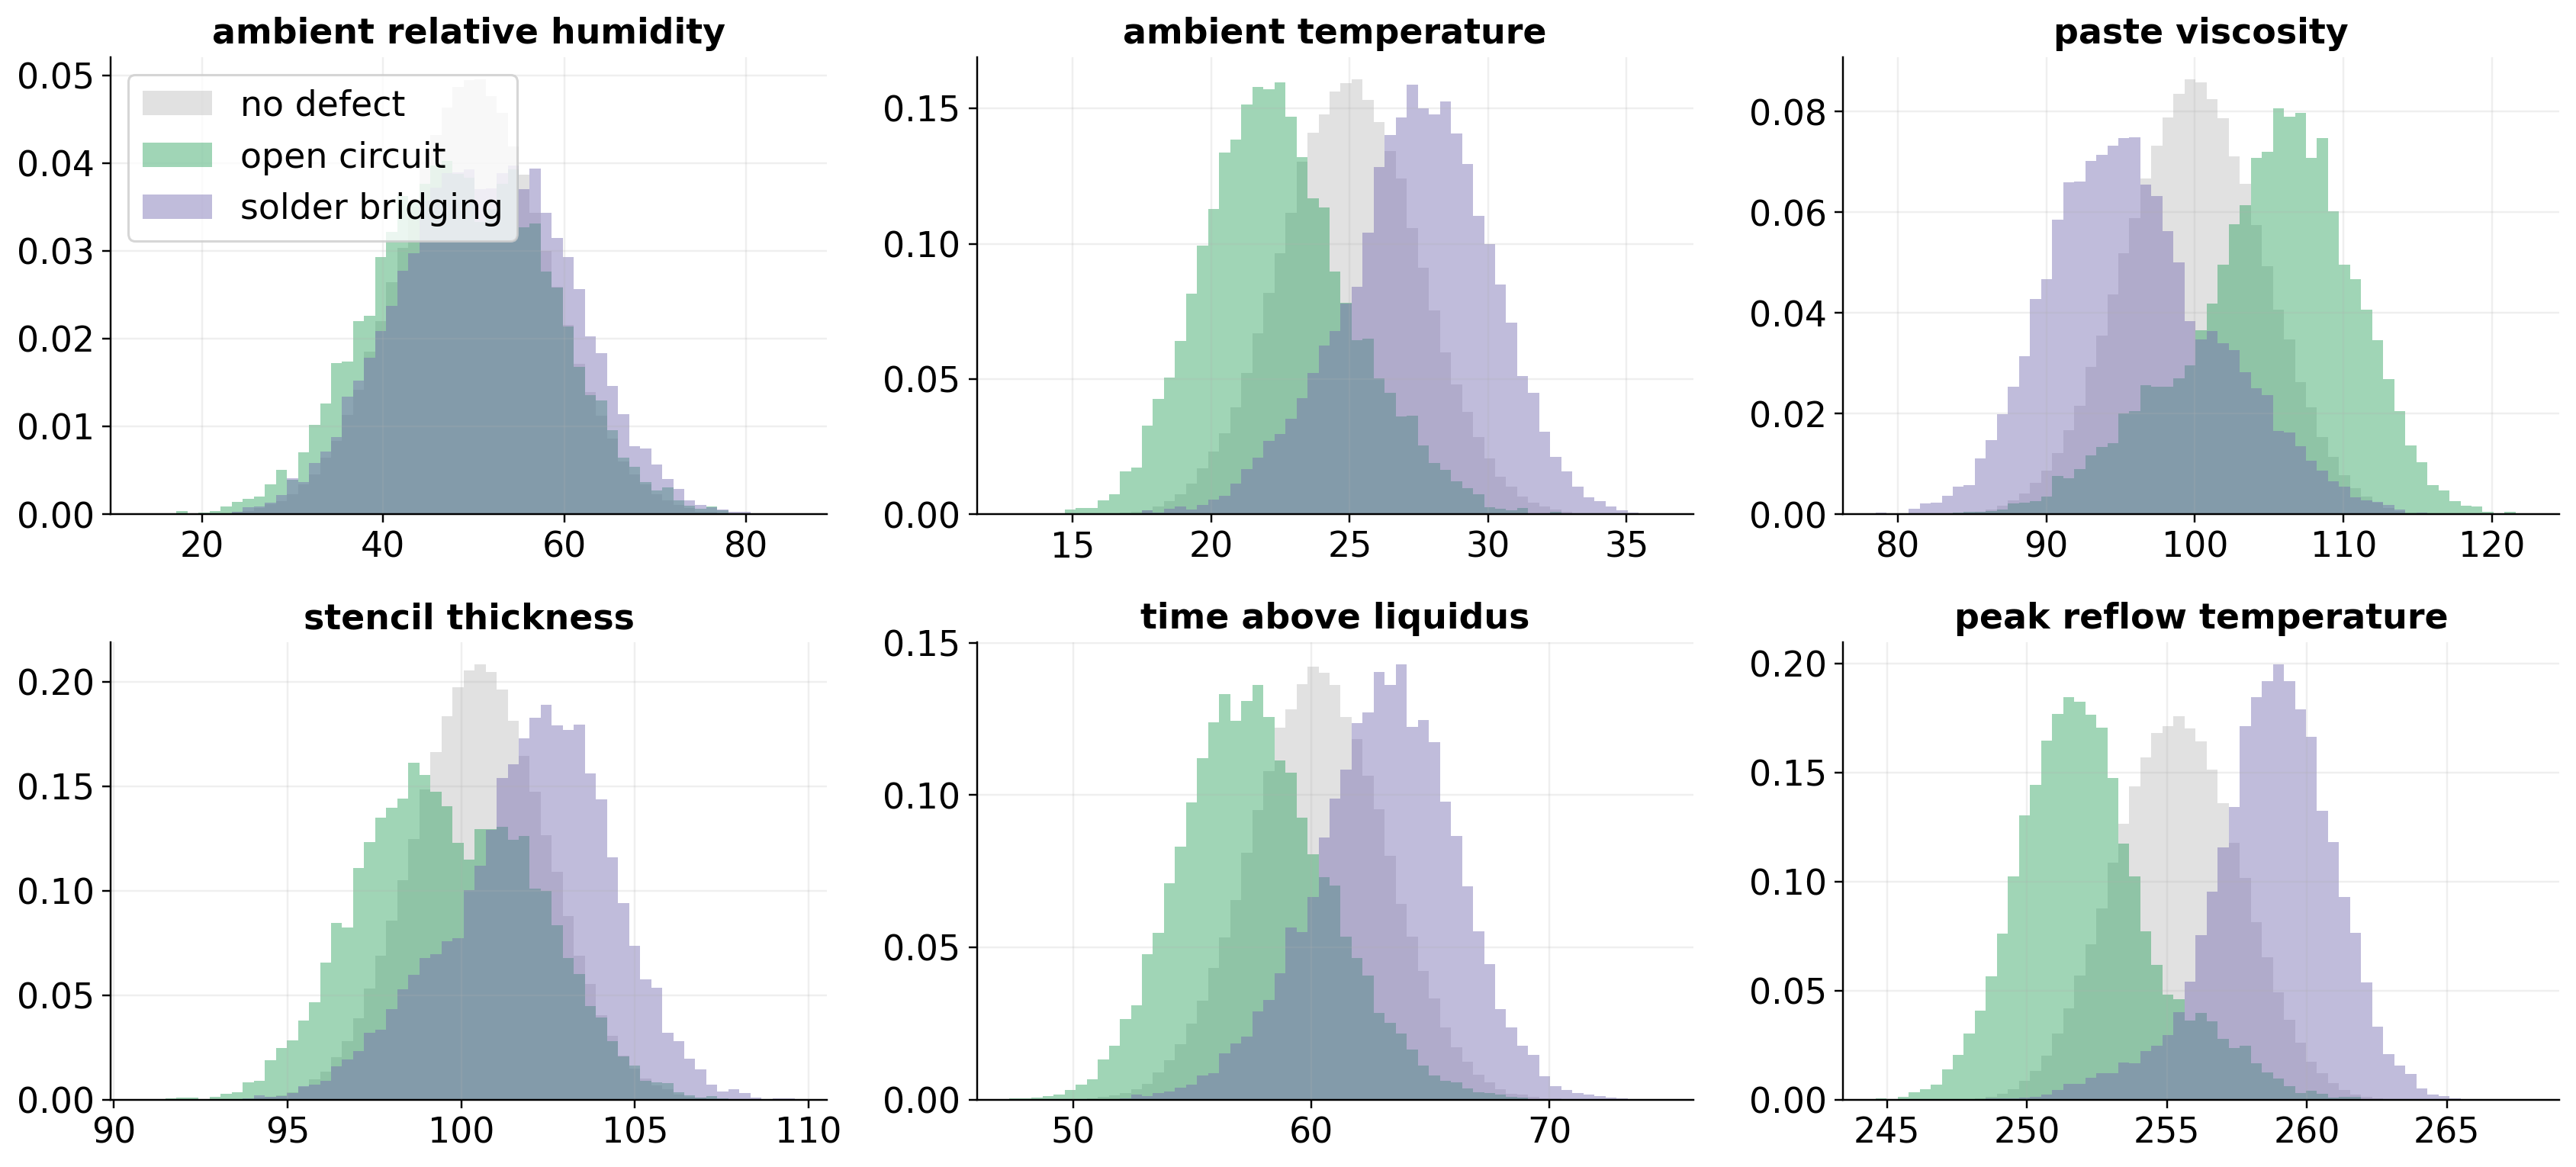
\includegraphics[width=\textwidth]{../tex/img/fig_feature_separability_baseline.png}
        \caption{Baseline.}
        \label{fig:baseline}
    \end{subfigure}

    \vspace{0.5em}

    \begin{subfigure}{.9\textwidth}
        \centering
        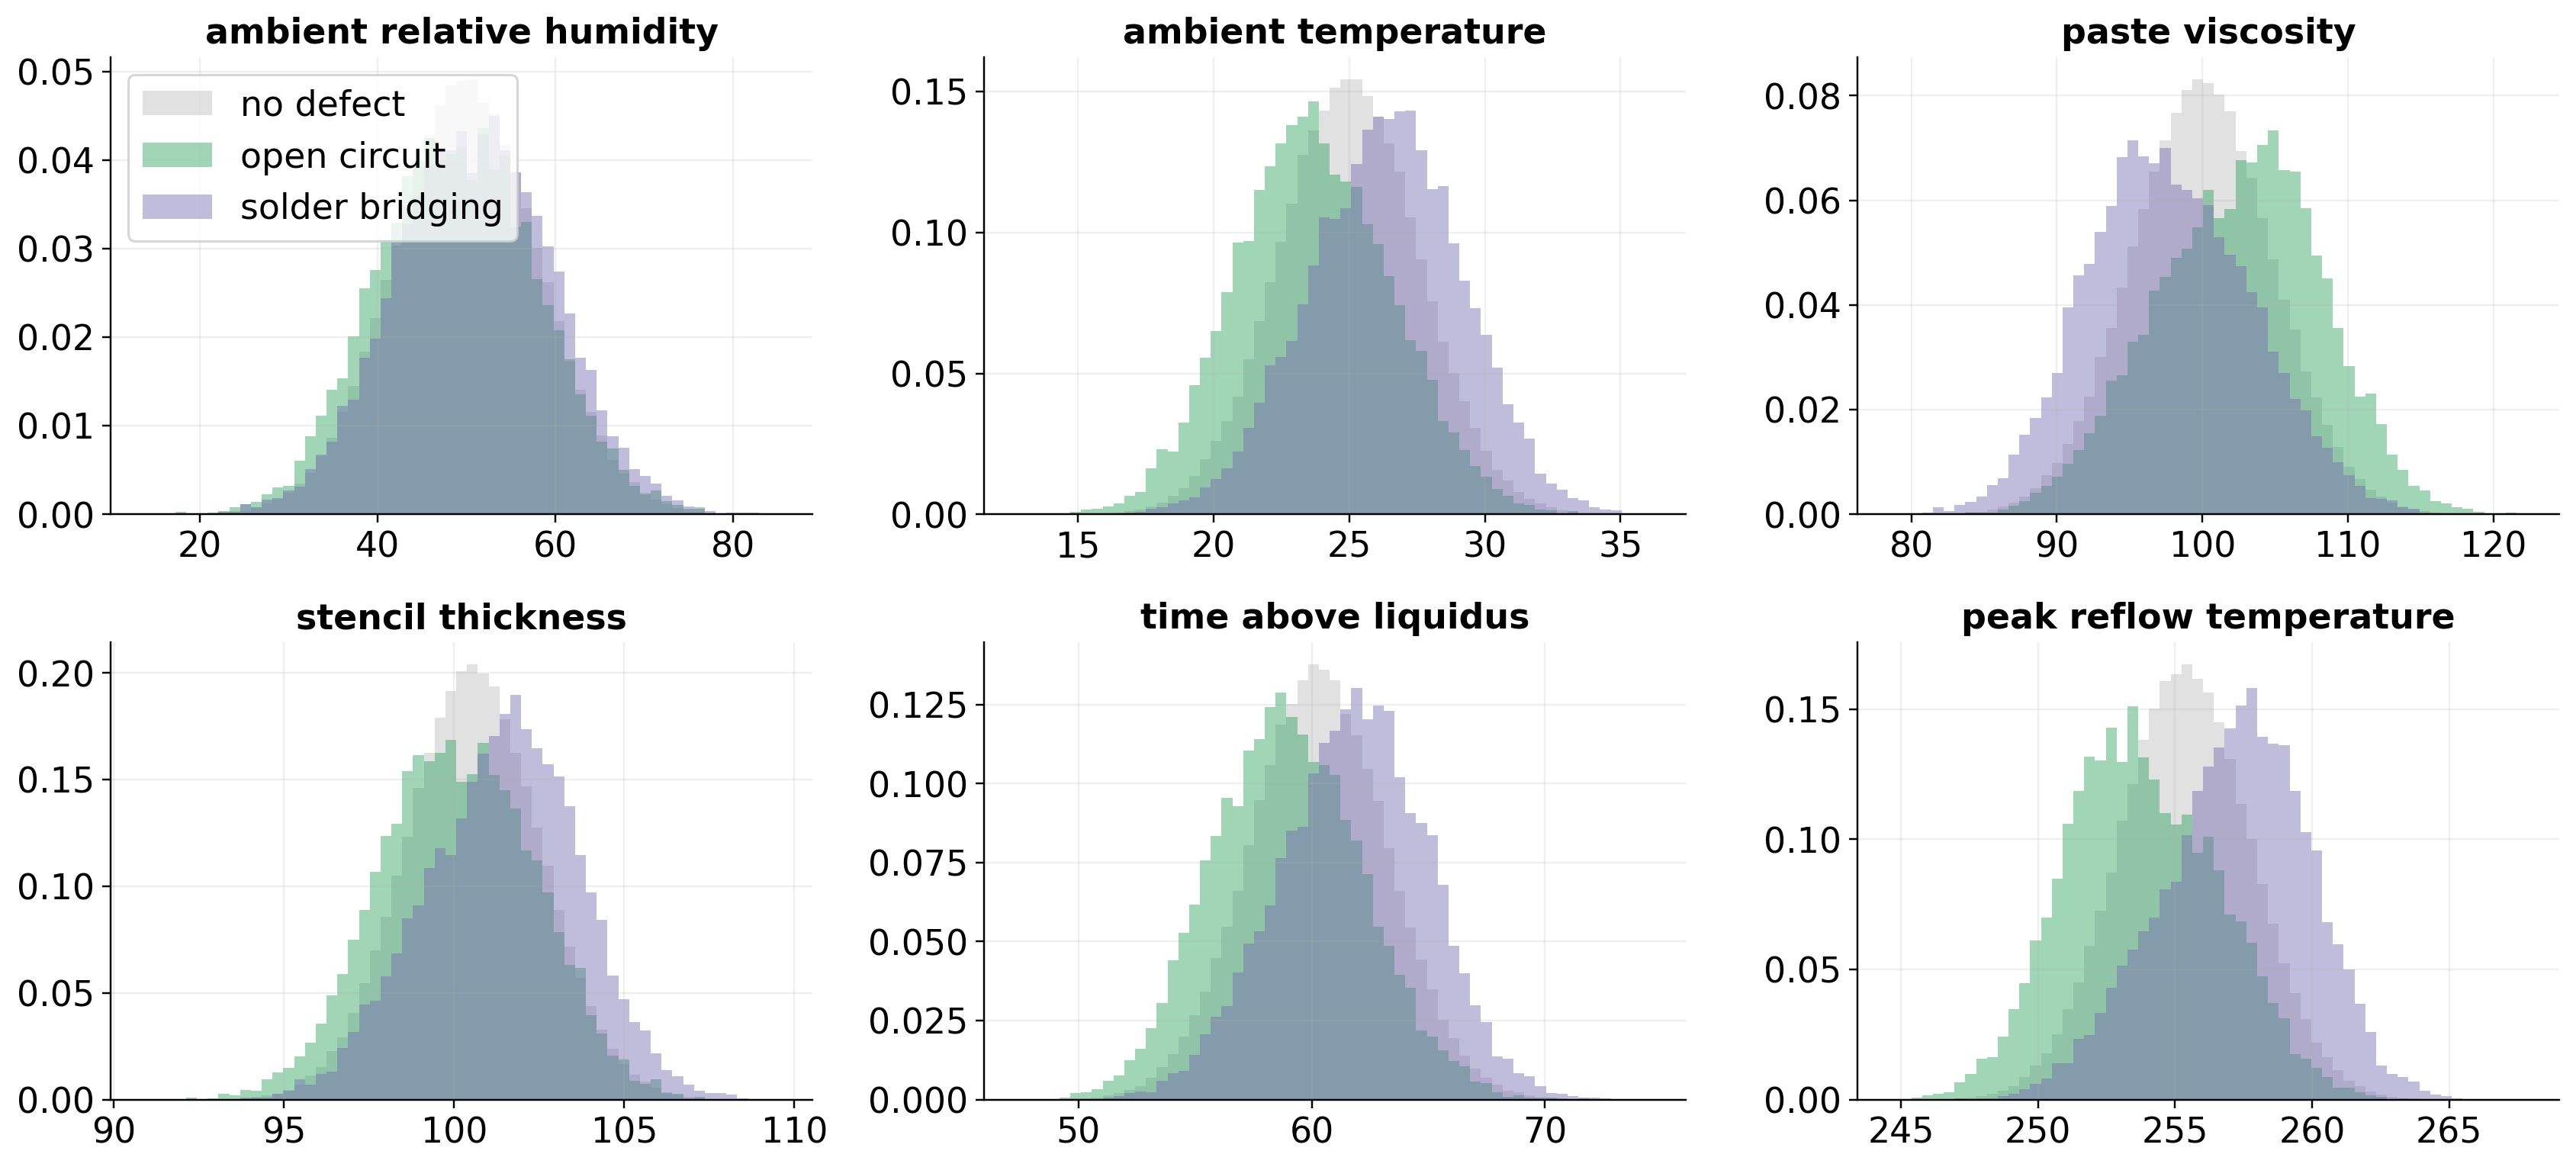
\includegraphics[width=\textwidth]{../tex/img/fig_feature_separability_harder.png}
        \caption{Increased class posterior overlap.}
        \label{fig:overlap}
    \end{subfigure}

    \caption{Feature distributions under different levels of class posterior overlap.}
    \label{fig:feature-separability}
\end{figure*}

\subsection{Experiment on real medical devices data}
\label{subsec:real-medical-devices-data}
\begin{enumerate}
    \item \raham{Plots with accuracy and risk curves should be done averaging over multiple seed and filling the area between +/- std curve.}
\end{enumerate}